\section{Umsetzung in HTML \& PHP}

\subsection{Seitenstruktur}

Alle Seiten der Anwendung sind nach dem gleichen Muster aufgebaut. Sie werden von der Datei \code{index.php} erzeugt. Hier werden wie in Abbildung \ref{fig:struktur} auf Seite \pageref{fig:struktur} die Seitenelemente aus den verschiedenen Include--Dateien für den Kopfbereich, die Navigationsleiste am rechten Rand und dem Fußbereich zusammengesetzt\footnote{Darstellung vereinfacht}. Der eigentliche Funktionsbereich\footnote{Frage anzeigen, Antworten speichern und auswerten, anmelden, abmelden, Eingabemaske für neue Fragen sowie das Abspeichern der neuen Fragen} werden von den PHP--Dateien im Verzeichniss \code{.../pages/} übernommen.

Diese Seitenelemente und Programmteile werden in einer Struktur aus \code{DIV}--Elementen angeordnet, welche durch die CSS--Klassen des Bootstrap--Frameworks zu einem modernen, responsiven Layout ausgezeichnet werden. Der Anwendungsentwickler braucht sich somit nicht um die optimale Darstellung der HTML--Seiten auf Desktoprechnern, Tabletts oder Smartphones zu kümmern. Jede Bildschirmgröße erhält durch Bootstrap automatisch ein speziell abgestimmtes Layout.

\section{Umsetzung in HTML \& PHP}

\subsection{Seitenstruktur}

Alle Seiten der Anwendung sind nach dem gleichen Muster aufgebaut. Sie werden von der Datei \code{index.php} erzeugt. Hier werden wie in Abbildung \ref{fig:struktur} auf Seite \pageref{fig:struktur} die Seitenelemente aus den verschiedenen Include--Dateien für den Kopfbereich, die Navigationsleiste am rechten Rand und dem Fußbereich zusammengesetzt\footnote{Darstellung vereinfacht}. Der eigentliche Funktionsbereich\footnote{Frage anzeigen, Antworten speichern und auswerten, anmelden, abmelden, Eingabemaske für neue Fragen sowie das Abspeichern der neuen Fragen} werden von den PHP--Dateien im Verzeichniss \code{.../pages/} übernommen.

\begin{figure}[h]
\begin{minted}[bgcolor=bg]{php}
<?php 
  include($_SERVER['DOCUMENT_ROOT'].'/includes/header.php'); 
?>
<div class="row">
 <div class="col-md-8">
  <?php 
    include($_SERVER['DOCUMENT_ROOT'].'/pages/'. $show . '.php'); 
  ?> 
 </div>
 <div class="col-md-4">
  <?php 
    include($_SERVER['DOCUMENT_ROOT'].'/includes/sidebar.php'); 
  ?>
 </div>	  
</div>
<?php 
  include($_SERVER['DOCUMENT_ROOT'].'/includes/footer.php'); 
?>
\end{minted}
\caption{HTML: Seitenstruktur und PHP--Includes}
\label{fig:struktur}
\end{figure}


Diese Seitenelemente und Programmteile werden in einer Struktur aus \code{DIV}--Elementen angeordnet, welche durch die CSS--Klassen des Bootstrap--Frameworks zu einem modernen, responsiven Layout ausgezeichnet werden. Der Anwendungsentwickler braucht sich somit nicht um die optimale Darstellung der HTML--Seiten auf Desktoprechnern, Tabletts oder Smartphones zu kümmern. Jede Bildschirmgröße erhält durch Bootstrap automatisch ein speziell abgestimmtes Layout.



\subsection{Layoutanpassungen mit CSS}




\begin{figure}[h]
\begin{center}
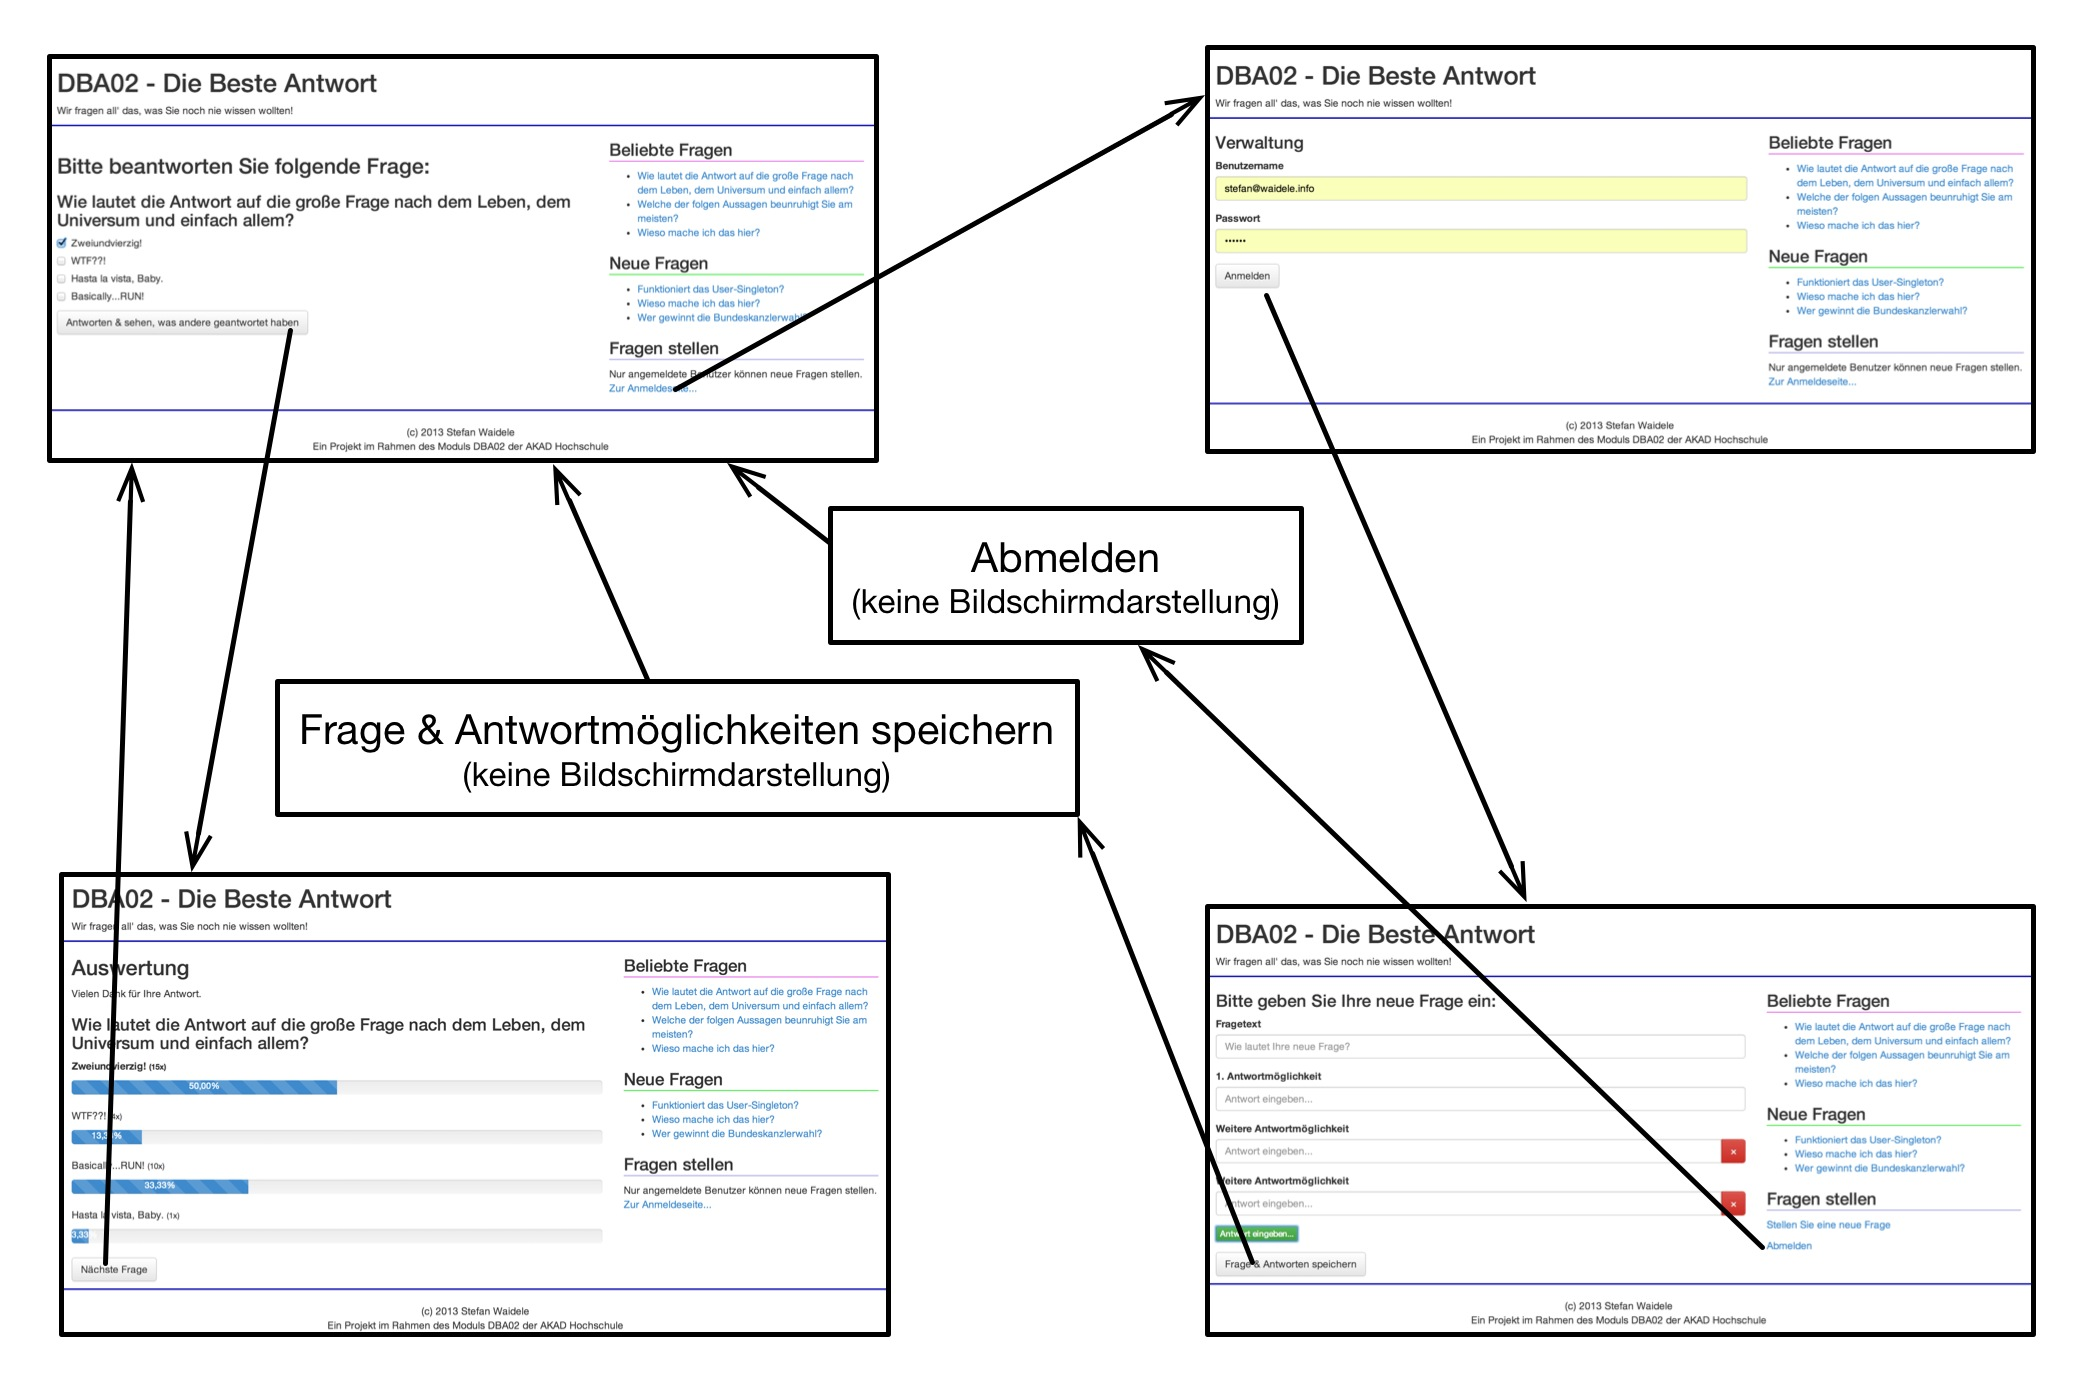
\includegraphics[width=\textwidth]{zustaende.jpg}
\caption{HTML--Seiten und Verlinkungen}
\end{center}
\label{fig:zustaende}
\end{figure}

